Real-time programming is about the acquisition and the processing of process variables of a technical process by means of digital programmable processors. 

    \begin{figure}[h]
    \centering
    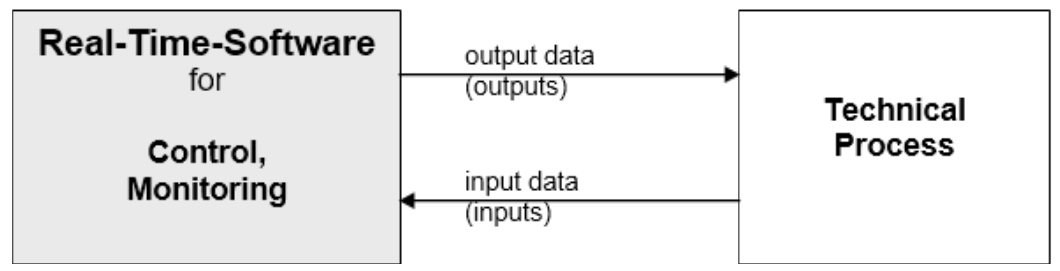
\includegraphics[width=10cm, height=2.5cm]{Images/image135.png}
    %\caption{}
    \label{fig:Fig 86}
    \end{figure}
    
For the acquisition of physical quantities, there are sensors, which convert a physical quantity to be measured into an electrical signal (a function of time).\\

\textbf{Analog signals}, are \textbf{continuous in value} (real valued) and they can be \textbf{continuous in time}, or \textbf{time discrete}. \\

\textbf{Digital signals} are \textbf{discrete in value}, and either \textbf{time discrete} or \textbf{continuous in time}.\\

Since \textbf{computers} can \textbf{process time discrete} and \textbf{value discrete signals} only, analog \textbf{sensor input signals} have to be converted into digital (\textbf{time and value discrete) signals}.

    \begin{figure}[h]
    \centering
    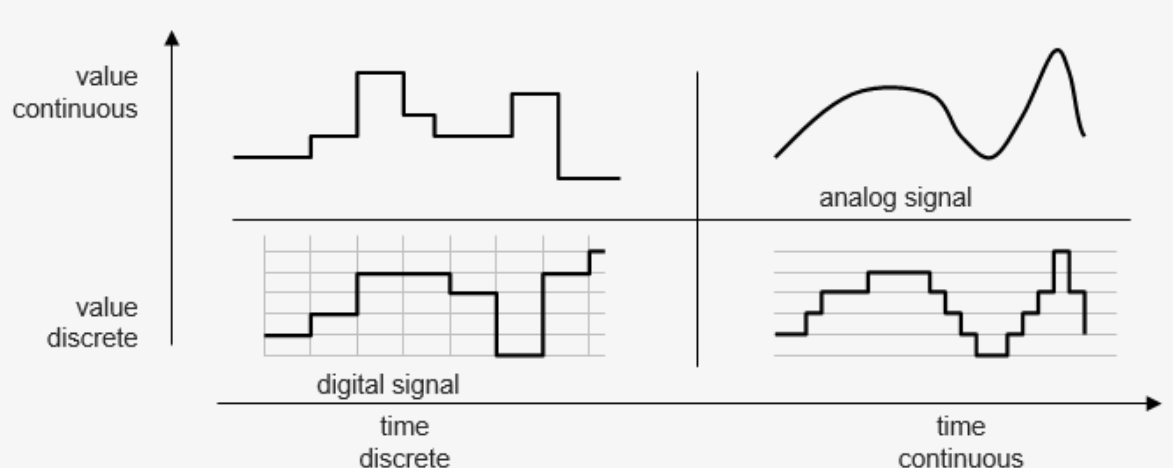
\includegraphics[width=14cm, height=5cm]{Images/image136.png}
    %\caption{}
    \label{fig:Fig 87}
    \end{figure}

Since a process can be affected by actuator, the \textbf{digital}, \textbf{time discrete} control signal, produced by a real-time computer program, must be converted back into an analog signal.

\section{Signal Conversion}

An analog sensor signal \textit{x}(\textit{t}) (time and value continuous) is first made time discrete by a sample-and-hold element. The sampling times are given from the I/O system of the computer. Analog signals are sampled at a constant sampling frequency \textit{f${}_{s}$} with sampling period \textit{T${}_{s}$} = 1${}_{\ }$/${}_{\ }$\textit{f${}_{s}$} .\\

It is usually ensured that the signal \textit{x}(\textit{t}) has no higher frequency components some limit frequency \textit{f${}_{g}$} $\mathrm{\le}$ 0.5·\textit{f${}_{s}$} . This is indicated by the analog low-pass filter with cutoff frequency \textit{f${}_{g}$}  sampling theorem see section 3.1.1.

    \begin{figure}[h]
    \centering
    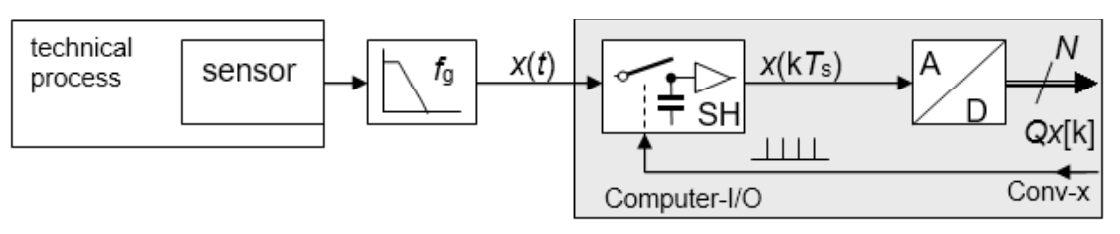
\includegraphics[width=15cm, height=3cm]{Images/image137.png}
    %\caption{}
    \label{fig:Fig 88}
    \end{figure}

The amplitudes of the signal \textit{x}(k·\textit{T${}_{s}$}) are still value continuous (real valued), but values change only at discrete times k·\textit{T${}_{s}$} (= \textbf{sampling}).\\

In a second step, the time discrete signal \textit{x}(k·\textit{T${}_{s}$}) is converted into a value discrete signal using an ADC (see section 4.5), i.e. the real value \textit{x} is approximated by an integer number \textit{Qx}, out of a sequence (0 {\dots} \textit{N}-1), such that \\

\textit{x} $\mathrm{\approx}$ \textit{Q${}_{x}$}·\textit{c${}_{x}$}       with \textit{c${}_{x}$} as some conversion factor  $\rightarrow$ (3.1).\\

After that \textit{Qx}[\textit{k}] is a digital signal (time- and value discrete) which can be stored and processes in the computer. With increasing time, the index k increases, e.g. the sequence $\mathrm{\{}$ \textit{Qx}[k-2], \textit{Qx}[k-1], \textit{Qx}[k] $\mathrm{\}}$ is the sequence of the last two recent and the actual sampling value. Example:\\

    \begin{figure}[h]
    \centering
    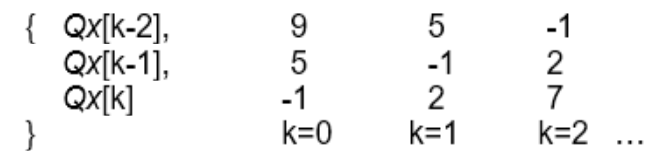
\includegraphics[width=6cm, height=2cm]{Images/image183.png}
    %\caption{}
    \label{fig:Fig 89}
    \end{figure}

a sequence \textit{Qx}[\textit{k}] as actual sampling value and with \textit{Qx}[\textit{k}-1] as the previous and \textit{Qx}[\textit{k}-2] as the pre-previous sample.\\

In the computer, the value discrete sequence \textit{Qx}[k] can be identified with the value continuous, time discrete sequence \textit{x}[k] and thus the analog signal \textit{x}(\textit{t}). \\

The quantization error \textit{e} = \textit{x} - \textit{Q${}_{x}$}·\textit{c${}_{x}$} with the sampling process can be minimized, since high resolution AD- and DA-converters are available
$\rightarrow$  \textit{e} can be usually neglected.

\subsection{Digital Sampling Systems}

Digital sampling systems are suitable for processing analog signals \textit{x}(\textit{t}) with discrete values as a time discrete sequence \textit{x}[k] = \textit{x}(k·\textit{T${}_{s}$}). \\

The original analog signal \textit{x}(\textit{t}) can be uniquely reconstructed from the time discrete sequence \textit{x}[\textit{k}], i.e. the original analog signal has a unique representation by the discrete sequence \textit{x}[\textit{k}]:\\

{\rot\bf Sampling Theorem of Shannon / Kotelnikov}

\begin{tcolorbox}[colback=blue!5!white,colframe=blue!75!black]
An analog signal sampled at constant frequency fs can be reconstructed from the discrete-time sequence of samples (up to a finite delay) if the bandwidth B is not greater than half the sampling frequency, thus B $<$ 0.5 fs.
\end{tcolorbox}

This is the fundamental theorem of digital signal processing.\\

If the bandwidth condition is violated, i.e. the bandwidth is greater than half the sampling frequency, the analog signal can not be uniquely reconstructed from the sampling, due to irreparable signal distortion, known as \textbf{aliasing}.\\

A digital sampling system, sampling at frequency \textit{f${}_{s}$} must ensure that an analog signal is bandlimited before sampling an upper frequency limit \textit{f${}_{g}$} $\mathrm{\le}$ 0.5\textit{ f${}_{s}$} .0.5\textit{ f${}_{s}$} is also called \textbf{Nyquist} \textbf{frequency} [3]. Thus, the sequence clearly determines the associated analog signal, which couldn't be processed by a digital computer directly!\\

(The proof is with another theorem of Fourier transform, stating that periodic sampling of a continuous time signal results in a periodic spectrum).\\

From the sampling theorem follows how the analog signal x(t-) can be reconstructed from the discrete time sequence \textit{x}[k]  by lowpass filtering of the discrete time signal:\\

    \begin{figure}[h]
    \centering
    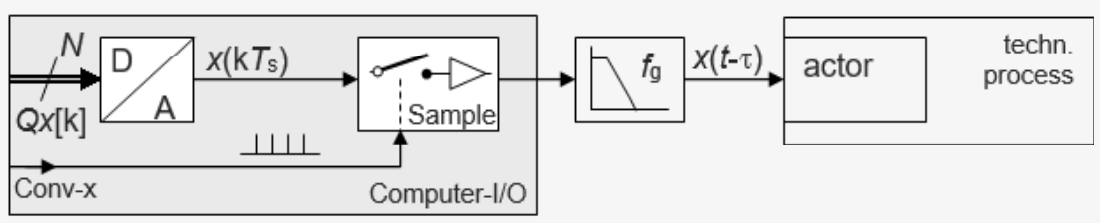
\includegraphics[width=14cm, height=2.5cm]{Images/image138.png}
    %\caption{}
    \label{fig:Fig 90}
    \end{figure}

The reconstruction is done by a periodic pulse train, sampling the DA converted, thus value discrete signal, which is finally (analog) lowpass filtered at cutoff frequency \textit{f}${}_{g}$ = 0.5$.$\textit{f}${}_{s}$\\ 

The output of the so-called "reconstruction lowpass" is \textit{x}(\textit{t}-), which is apart from a certain constant time delay  the analog signal \textit{x}(\textit{t}) !\\

{\rot\bf Real-Time Conditions for Sampling Systems}\\

It is of great importance importance for signal quality, that strict periodicity of the sampling period. Any deviations from strict periodicity acts as signal interference, which may have some unpredictable consequences with closed loop sampling controllers (e.g. instable control).\\

A typical requirement for max. \textbf{jitter} (average deviation) of sampling period is 0.1\% to 1\%.

\begin{tcolorbox}[colback=blue!5!white,colframe=blue!75!black]
With digital sampling systems
\begin{enumerate}
\item strict periodicity of the sampling process in both the AD and the DA conversion
\item to comply with the Nyquist condition (the analog lowpass filters - before any ADC and -after any DAC- with the right cutoff frequency)
\end{enumerate} 	
shall be respected.
\end{tcolorbox}

Digital signal processing of analog signals involves very strict requirements to real-time conditions of some software tasks, due to the periodic and exact sampling conditions.

\begin{table}[h!]
\setlength{\tabcolsep}{10pt} % Default value: 6pt
\renewcommand{\arraystretch}{1.5} % Default value: 1
\small
\centering
 \begin{tabular}{|c|c|c|c|} \hline
 \textbf{Action} & \textbf{Time Condition} \\ [0.1ex] 
input of a sample of an analog signal &  \\ \hline 
computation of a signal sample &  \\ \hline 
output of the calculated signal sample &  \\ \hline 
 \end{tabular}
 %\caption{\textbf{}}
 \label{Intrinsic}
\end{table}

\textbf{ Example}: Sampling Control (Digital Control) as real-time application using 2 Tasks and 2 Queues

    \begin{figure}[h]
    \centering
    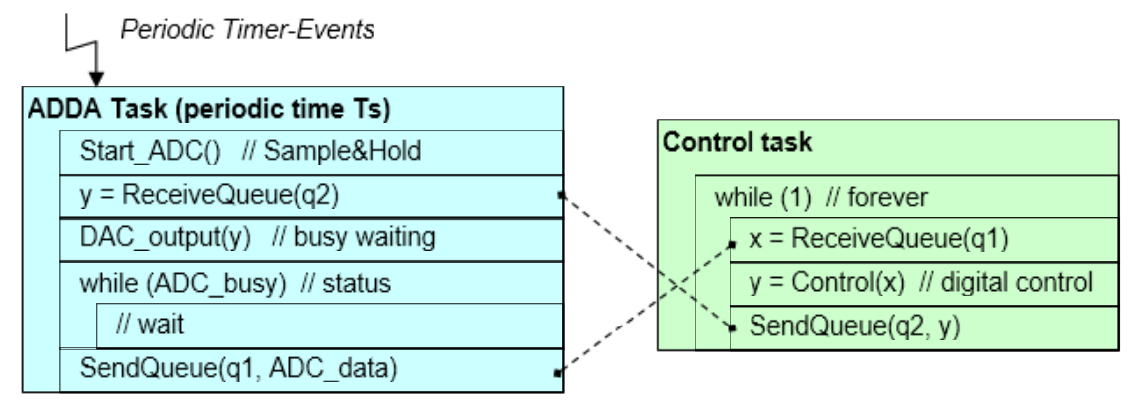
\includegraphics[width=14cm, height=5cm]{Images/image139.png}
    %\caption{}
    \label{fig:Fig 91}
    \end{figure}

*the Queue q2 must be initialized, before the ADDA Task starts.\\

Instead of a queue, often just a semaphore is used for synchronization \\

\textbf{Negative Example}: Not appropriated due to differences in run-time  jitter !!

\begin{itemize}
\item $\rightarrow$ Non deterministic sampling \\ Violation of the exact real-time condition !!
\item $\rightarrow$ Samples cannot be reconstructed, \\ Distortions and Artefacts with (HQ) Multimedia signals
\item $\rightarrow$ Stability of a closed-loop control is in danger, cannot been guaranteed !!
\end{itemize}

    \begin{figure}[h]
    \centering
    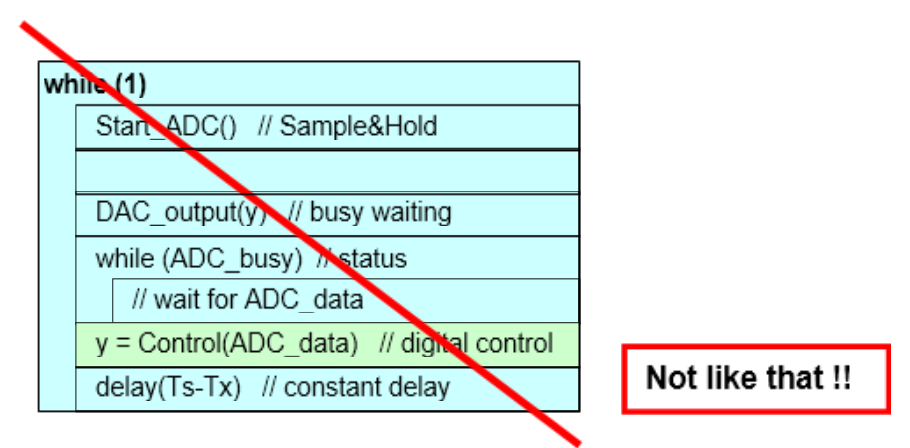
\includegraphics[width=10cm, height=4.5cm]{Images/image184.png}
    %\caption{}
    \label{fig:Fig 92}
    \end{figure}
\newpage
{\rot\bf Quantization}\\

A discrete-time signal \textit{x}(k·\textit{T${}_{s}$}) is quantized using an AD converter, i.e. its value (amplitude) is approximated by an integer number with \textit{N} discrete values. This is because a digital computer can handle value discrete (integer) values only, not value-continuous (real) values.\\

The number of values \textit{N} are often powers of two, i.e. \textit{N} = 2\textit{${}^{M}$}, so one obtains an \textit{M}-bit AD conversion, with the conversion factor \textit{c${}_{x}$}, which gives the value of an LSB (least significant bit) as a physical quantity\\

\begin{equation}
	\begin{array}{l} {x_{Q} =Qx\cdot c_{x} +x_{\min } =Qx\cdot \frac{x_{\max } -x_{\min } }{N} +x_{\min } } \\
	
	 {c_{x} =\frac{x_{\max } -x_{\min } }{N} =\frac{x_{\max } -x_{\min } }{2^{M} } } \end{array}
\label{EQ }
\end{equation}

Qx	integer representation of x\\
xQ	quantized physical quantity\\
cx	conversion factor\\

In automation 8-, 10-, 12-, 14- bit AD converters are used more often than, say, 16-, 20- or 24-bit ADCs, the latter are mainly used for audio signals.\\

The deviation e = \textit{x${}_{Q}$} - \textit{x} is called quantization error. In most applications, the number of conversion stages is \textit{N} are chosen high enough, such that the quantization error is negligible, then \textit{x${}_{Q}$} = \textit{x}.\\

\textbf{Example}: A pressure sensor with an 8-bit AD converter is equipped for a measuring a pressure signal with a range of values (\textit{p${}_{min}$}, \textit{p${}_{max}$}) = (0, 1500) mbar.\\

The conversion factor by \eqref{GrindEQ__3_1_} is \textit{c${}_{p}$} = 1500 mbar / 2${}^{8}$ = 5.86 mbar.\\

The quantization of the sensor signal is a step function with a linear increase. The value change takes place usually with a so-called \textbf{\textit{mid tread}} pattern, i.e., in the middle of an interval.\\

    \begin{figure}[h]
    \centering
    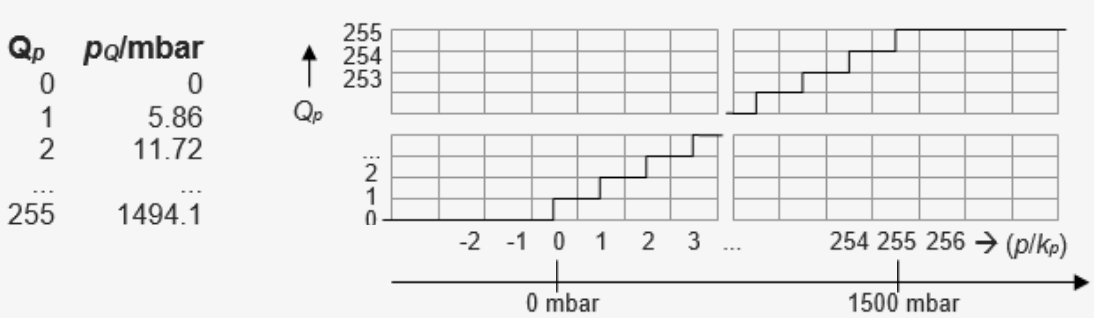
\includegraphics[width=12cm, height=4.5cm]{Images/image141.png}
    %\caption{}
    \label{fig:Fig 93}
    \end{figure}

The pressure signal is to be scanned by a process computer at a sampling frequency of 10 Hz. A warning signal at a low pressure \textit{p}${}_{L}$ = 0.7 bar and at overpressure \textit{p}${}_{H}$ = 1.2 bar shall be issued.\\

The bandwidth of the analog low-pass filter must be less than 5 Hz!\\

An appropriate real-time program for a microcontroller shall be designed with two tasks: 1. a task for pressure signal acquisition, 2. analysis and output.\\

\textbf{Possible Solution}: 2 Tasks in an FPN schedule:

\begin{itemize}
\item \textbf{task 1}:  \textit{T}${}_{p1}$ = 100 ms, (sampling jitter $<$  0.1 ms). Acquisition of values \textit{Qp}, setting the semaphore S1, if a new value Q\textit{p}[n] is available.

\item \textbf{task 2}:  wait for S1, then \\
(a) evaluate \textit{Qp}[n]:  compare with the lower limit\\
\textit{Qp}${}_{min}$ = round(\textit{p}${}_{min}$ / k${}_{P}$) = round(700 mbar / 5.86 mbar) = 119\\
set Output\_pmin, if (x[n] $\mathrm{<}$ \textit{Qp}${}_{min}$)\\

(b) evaluate \textit{Qp}[n]: compare with the upper limit  \\  \textit{Qp}${}_{max}$ = round(\textit{p}${}_{max}$ / k${}_{P}$) = round(1200 mbar / 5.86 mbar) = 205 \\ set Output\_pmax, if (x[n] $\mathrm{>}$ \textit{Qp}${}_{max}$)
\end{itemize}

    \begin{figure}[h]
    \centering
    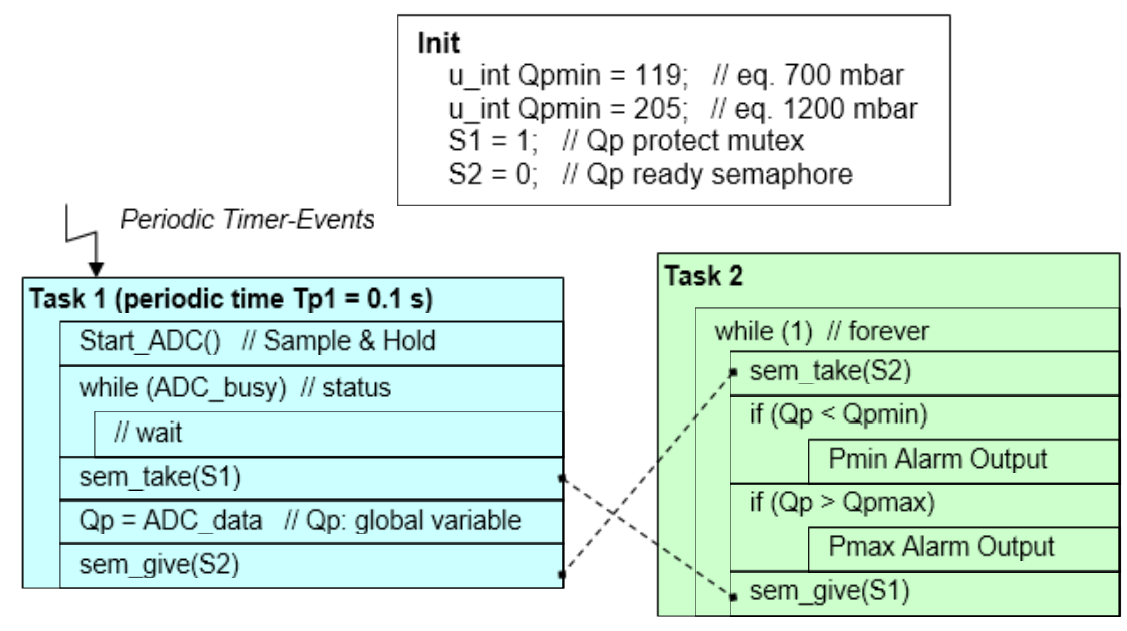
\includegraphics[width=12cm, height=7cm]{Images/image142.png}
    %\caption{}
    \label{fig:Fig 94}
    \end{figure}

\section{Digital Filters}

Linear digital filters can be described as LTI-Systems (\textbf{l}inear, \textbf{time-i}nvariant) by means of difference equations. The general form of a linear difference equation with constant, real coefficients \textit{a${}_{j}$},\textit{b${}_{j}$} is

\[a_{0} y[n]+a_{1} y[n-1]+a_{2} y[n-2]+......+a_{N} y[n-N]=b_{0} x[n]+b_{1} x[n-1]+b_{2} x[n-2]+....+x_{M} u[n-M]\] 
\[\sum _{j=0}^{N}a_{j} \cdot y[n-j] =\sum _{j=0}^{M}b_{j} \cdot x[n-j] \] 

it is always possible to define \textit{a}${}_{0}$ = 1, which results in a  recursion formula for the actual output value with constant coefficients \textit{a${}_{j}$},\textit{b${}_{j}$}

\begin{equation}
	y[n]=\quad \sum _{j=0}^{M}b_{j} \cdot x[n-j] \; \; \, -\sum _{j=1}^{N}a_{j} \cdot y[n-j]\ with\ \textit{a}{}_{0} = 1\ (by convention)
\label{EQ }
\end{equation}

    \begin{figure}[h]
    \centering
    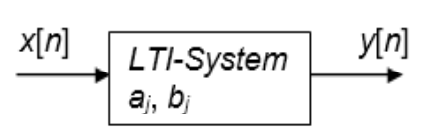
\includegraphics[width=5cm, height=1.5cm]{Images/image185.png}
    %\caption{}
    \label{fig:Fig 95}
    \end{figure}

{\rot\bf Structure of the general LTI-System}

    \begin{figure}[h]
    \centering
    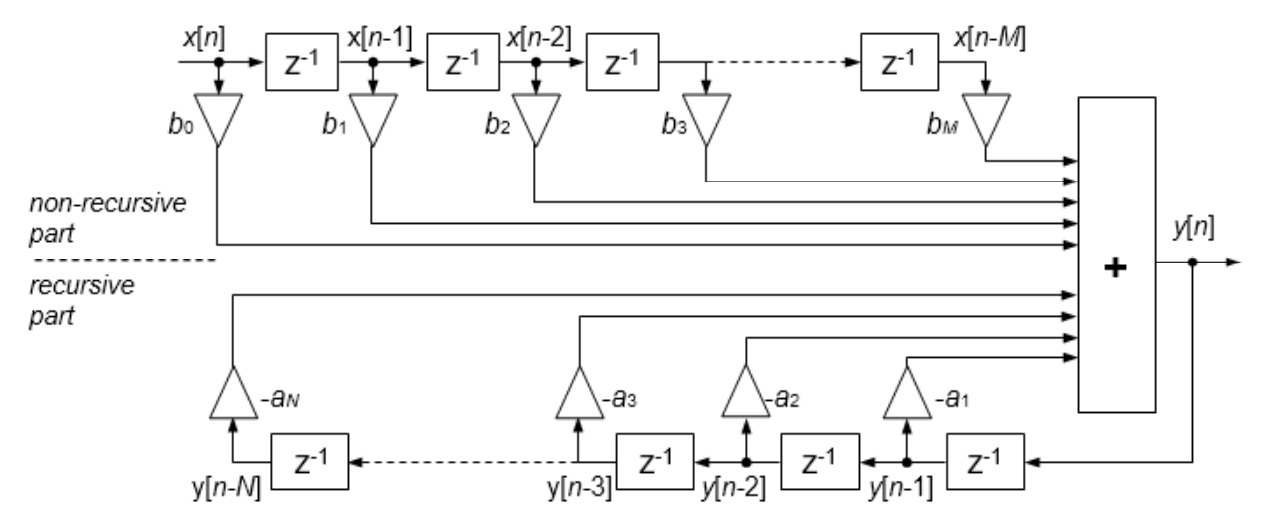
\includegraphics[width=14cm, height=5.5cm]{Images/image143.png}
    %\caption{}
    \label{fig:Fig 96}
    \end{figure}

The z${}^{-1}$ rectangles symbolize a delay by one sample in time, the triangles symbolize a multiplication with a constant. The denominator degree \textit{N} is also known as filter order. There are 2 basic types of digital filters 

\begin{enumerate}
\item  recursive filters with \textbf{IIR}-behavior (\textbf{i}nfinite \textbf{i}mpulse \textbf{r}esponse), with \textit{N} $\mathrm{>}$ 0

\item  non-recursive filters with \textbf{FIR}-behavior (\textbf{f}inite \textbf{i}mpulse \textbf{r}esponse), with \textit{N} = 0
\end{enumerate}

With each new sampling period (increment of index \textit{k}) a new output value \textit{y}[\textit{n}] can be started earliest after the availability of a new input value \textit{x}[\textit{n}], and the calculation needs to be finished before the next sampling period (Deadline !)  see 3.1.1\\

For Integer implementations it is often economical to scale the difference equation \eqref{GrindEQ__3_2_} with am appropriate factor S such, that the multiply and add operations can be realized with integer arithmetic operations, most microcontroller CPUs support (rather than floating point arithmetic, which is common to larger, powerful CPUs):

\begin{equation}
	y[n]=\quad \frac{\sum _{j=0}^{M}(Sb_{j} )\cdot x[n-j] \; \; \, -\sum _{j=1}^{N}(Sa_{j} )\cdot y[n-j] }{S} =\frac{A}{S}   ,  \hspace{2cm}  \textit{S} \in \textbf{N}
\label{EQ }
\end{equation}

The coefficients \textit{Sb${}_{j}$ }and \textit{Sa${}_{j}$} can be represented with sufficient precision by integer numbers, if S is chosen large enough. Since input- and output sequence values \textit{x}[] and \textit{y}[] are also integers, the numerator in \eqref{GrindEQ__3_3_} can be evaluated using integer-multiplication and -addition using an \textbf{\textit{accumulator}} \textit{A} with increased width (i.e. len x,y: 16-bits, len A: 64 bit). 

Particularly effective as a choice for S = 2\textit{${}^{ldS}$} is a power of 2, thus the final division by N can be replaced by an equivalent right-shift operation  

\begin{equation}
	\frac{A}{S}      (\textit{A} >> \textit{ldS})  \hspace{1cm}    without\ round\ op. \nonumber
\label{EQ }
\end{equation}

\begin{equation}
	\frac{A+S/2}{S}     (\textit{A} + S/2) >> \textit{ldS}  \hspace{1cm}  with\ round\ op. \nonumber
\label{EQ }
\end{equation}

{\rot\bf Rules for Optimizing Execution Time on Standard-Microcontrollers}\\

Since most standard micro-controller CPUs do not support floating point arithmetic in hardware, and also lack for a full division (modulo) hardware support, these functions are implemented by means of software libraries.With critical CPU load, a code optimization is useful to reduce the WCET of any computationally intensive task. Particularly effective measures are

\begin{enumerate}

\item  Avoiding add/sub and multiplication (float, double) \\$\rightarrow$scaling by a power of two, and multiply with integers \\ Exception: floating point operations are fine, if supported by the hardware.

\item  Avoiding of Division (/)\\$\rightarrow$ Right Shift ($\mathrm{>}$ $\mathrm{>}$) with powers of two instead of division

\item  Avoiding of Modulo (\%) \\$\rightarrow$ Bitwise AND (\&) with powers of two instead of modulo

\item  Review of the assembly based on the compiler list files (based on the specified CPU cycles) for execution time critical code
\end{enumerate}

{\rot\bf Example Digital IIR-Lowpass 1. Order }\\

$y[n]=b_{0} \cdot x[n]\; \, -a_{1} \cdot y[n-1]$ $y[n]=b_{0} \cdot x[n]\; \, -a_{1} \cdot y[n-1]$ \\

Given:   filter-coefficients: \textit{b}${}_{0}$ = 0.3333, \textit{a}${}_{1}$ = -0.6667. \\
Wanted:  impulse-response and step-response for \textit{n} $\mathrm{\ge}$ 0.     C-realization with float- and integer- (fixed-point) arithmetic.

\begin{itemize}
\item \textbf{Impulse response}  \textit{x}[\textit{n}] = [\textit{n}]:   \textit{x} = { 1, 0, 0, 0, ...}
    \begin{figure}[h]
    \centering
    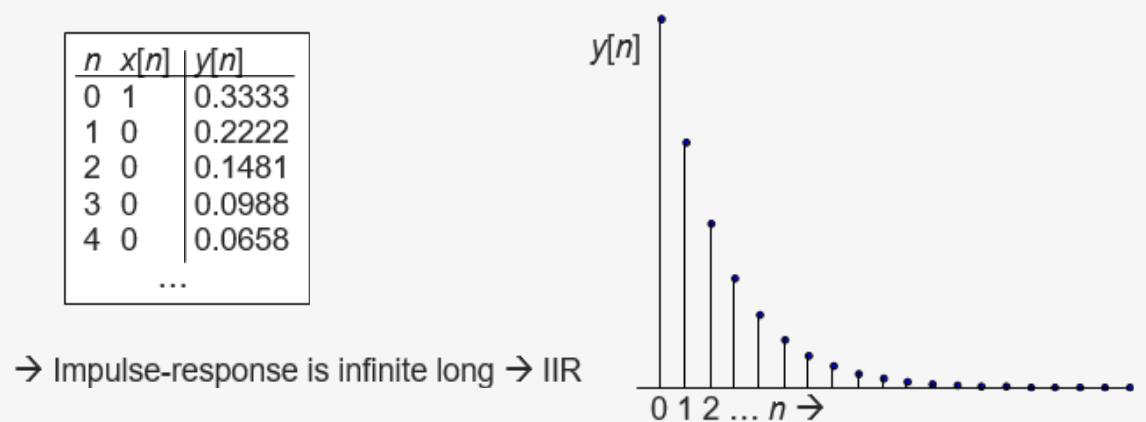
\includegraphics[width=12cm, height=4cm]{Images/image144.png}
    %\caption{}
    \label{fig:Fig 97}
    \end{figure}

Impulse-response is infinite long \hspace{1cm} $\rightarrow$ IIR

\item \textbf{Step-response} \textit{x}[\textit{n}] = [\textit{n}]:   \textit{x} = {1, 1, 1, 1, ...}
	\begin{figure}[h]
    \centering
    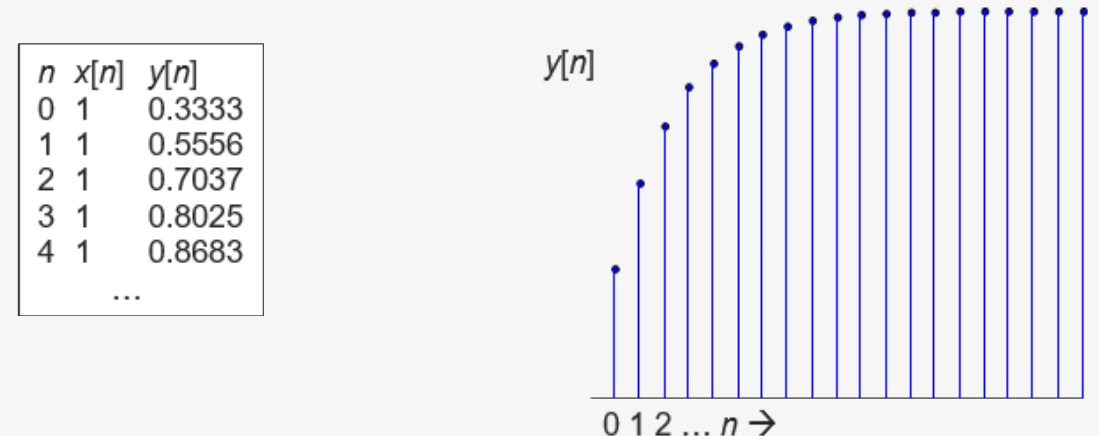
\includegraphics[width=12cm, height=4cm]{Images/image145.png}
    %\caption{}
    \label{fig:Fig 98}
    \end{figure}

$\rightarrow$ The step-response approximates the value 1.0 for large \textit{n}, as expected.
\end{itemize}

{\rot\bf C- Realization (float): } \\

On microcontrollers without float-hardware needs hundreds of machine cycles and is thus very un-effective ( section 3.2.1) !
\newpage
	\begin{figure}[h]
    \centering
    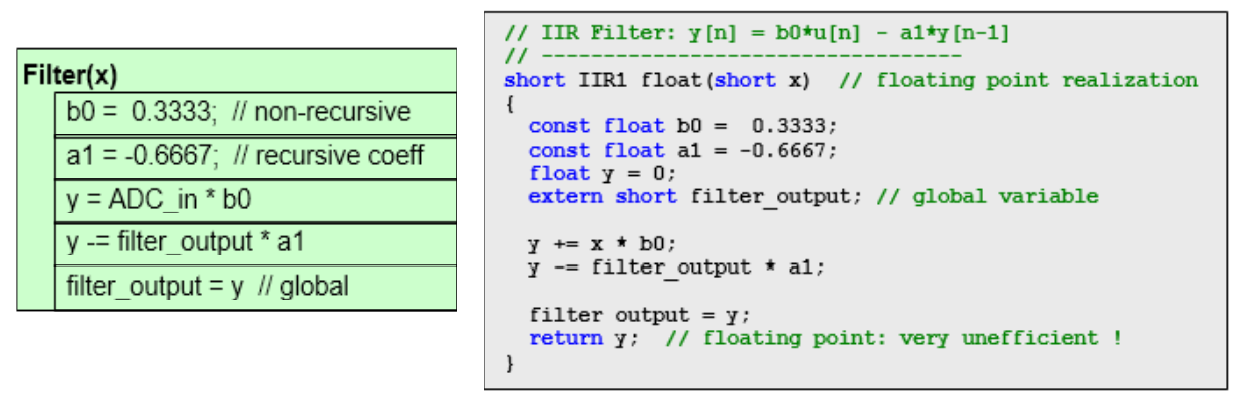
\includegraphics[width=14cm, height=4cm]{Images/image146.png}
    %\caption{}
    \label{fig:Fig 99}
    \end{figure}

{\rot\bf C- Realization (integer): } \\

Using the integer difference equation \eqref{GrindEQ__3_3_} with a power of 2: \textit{S} = 2\textit{${}^{ldS\ }$}

\[\begin{array}{l} {S\cdot y[n]=(Sb_{0} )\cdot x[n]-(Sa_{1} )\cdot y[n-1]} \\ {Sb_{0} =S\cdot 0.3333} \\ {-Sa_{1} =S\cdot 0.6667} \end{array}\] 
 
For example, if \textit{ldS} = 12 is chosen, S = 2${}^{12}$ = 4096 follows

\[\begin{array}{l} {4096\cdot y[n]=1365\cdot x[n]-(-2761)\cdot y[n-1]} \\ {\qquad Sb_{0} =1365} \\ {\qquad Sa_{1} =-2731} \\ {y[n]=\frac{1365\cdot x[n]+2761\cdot y[n-1]}{4096} =\frac{A}{4096} \approx (A>>12)} \end{array}\] 

Thus, with the scaled difference equation the \textit{S}-fold result is calculated and stored in the accumulator \textit{A}. Instead of dividing \textit{A} by \textit{S}, the effective right-shift operation (here: $\mathrm{>}$ $\mathrm{>}$ 12) is used.

	\begin{figure}[h]
    \centering
    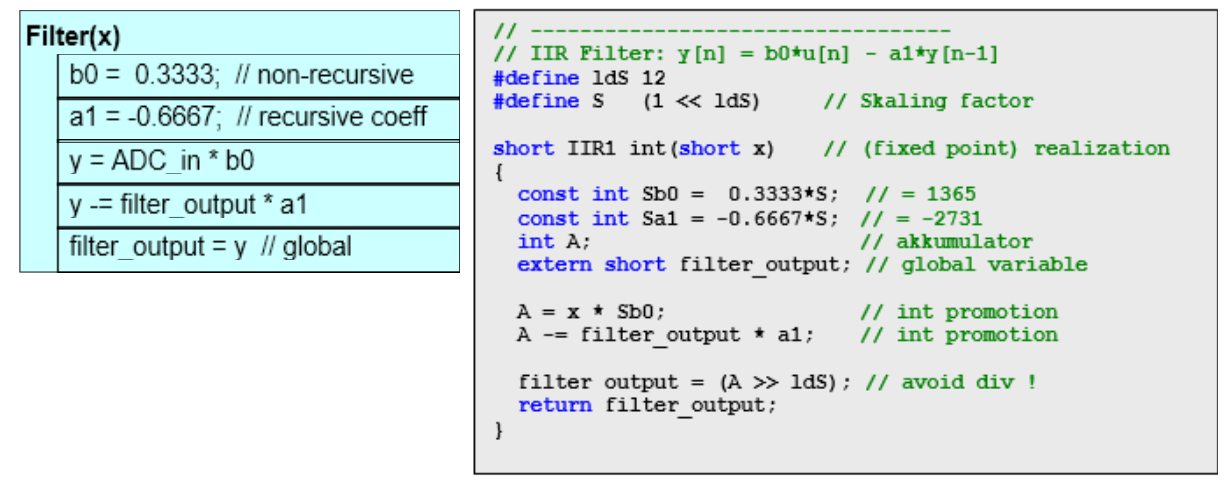
\includegraphics[width=14cm, height=5.5cm]{Images/image147.png}
    %\caption{}
    \label{fig:Fig 100}
    \end{figure}

Even on microcontrollers without float-hardware, but hardware multiplyer for integers utilizes only a handful of machine cycles and thus is very effective (on AVR ca. factor 100 faster than the float-version) !
\newpage
\section{Digital Controls}

{\rot\bf PID Controller}\\

For many control systems in engineering, controls are used, which follow the so-called PID (\textbf{P}roportional-\textbf{I}ntegral-\textbf{D}ifferential) principle. Each of the 3 controller parts has its term with a specific parameter \textit{k${}_{R}$,} \textit{T${}_{N}$}, and \textit{T${}_{V}$} which allow the system response to be optimized with respect to stability, or under the influence of disturbances

	\begin{figure}[h]
    \centering
    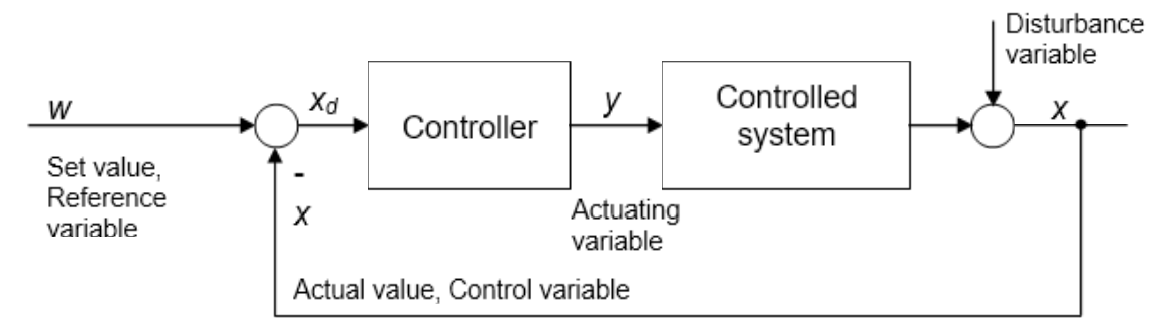
\includegraphics[width=14cm, height=4cm]{Images/image148.png}
    %\caption{}
    \label{fig:Fig 101}
    \end{figure}

{\rot\bf System behavior of an analog PID Controller}\\

\begin{equation}
	 y(t)=K_{R} \cdot \left[x_{d} (t)+\frac{1}{T_{N} } \int x_{d} (t)\, dt+T_{V}  \frac{dx_{d} (t)}{dt} \right]
\label{EQ }
\end{equation}

For an analog PID controller the circuit principle below was chosen in the past, the parameters were often calculated approximately. Finally, with the complete system, the parameters were finely adjusted empirically by adjustment of the balancing resistors.

	\begin{figure}[h]
    \centering
    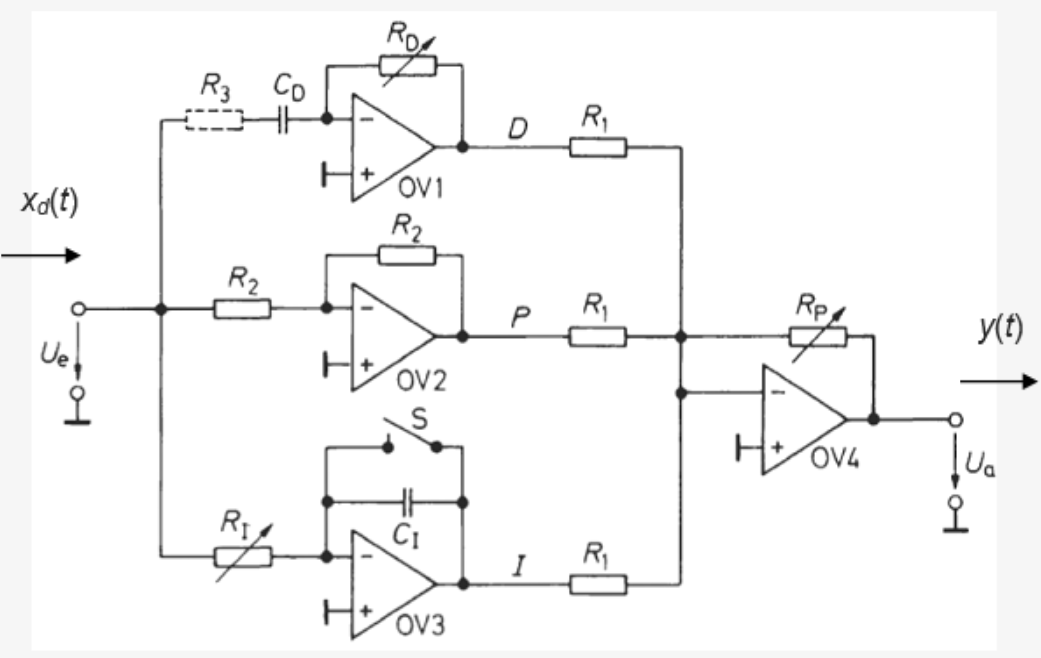
\includegraphics[width=12cm, height=5.5cm]{Images/image149.png}
    %\caption{}
    \label{fig:Fig 102}
    \end{figure}

dimensioning:$k_{R} =\frac{R_{p} }{R_{1} } ,\, \, \, T_{N} =R_{I} \cdot C_{I} ,\, \, \, T_{V} =R_{D} \cdot C_{D} $     [Tietze]\\

The PID controller behavior \eqref{GrindEQ__3_4_} can be simulated using a digital sampling system with a suitable control algorithm invoked periodically with the sampling period \textit{T${}_{s}$}. The derivation is shown in [Oppen] oder [Kamm]:

	\begin{figure}[h]
    \centering
    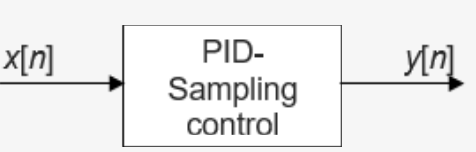
\includegraphics[width=5cm, height=2cm]{Images/image150.png}
    %\caption{}
    \label{fig:Fig 103}
    \end{figure}

\textbf{Standard PID Regler Algorithmus}  ([LutzW] p. 477)

\begin{equation}
	\begin{array}{l} {y[n]=y[n-1]+} \\ {\, \, \, \, \, \, \, \, \, \, \, \, \, K_{R} \cdot \left[x[n]\cdot \left(1+\frac{T_{V} }{T_{S} } \right)-x[n-1]\cdot \left(1-\frac{T_{S} }{T_{N} } +2\frac{T_{V} }{T_{S} } \right)+x[n-2]\cdot \frac{T_{V} }{T_{S} } \right]} \end{array}
\label{EQ }
\end{equation}

{\rot\bf PI-Controller }\\

If the time constant \textit{T${}_{V}$} of the differential term is set to 0 in \eqref{GrindEQ__3_5_}, the algorithm for the PI-controller is obtained, which has a proportional- and an integral term only:

\begin{equation}
	y[n]=y[n-1]+\, K_{R} \cdot \left[x_{d} [n]-x_{d} [n-1]\cdot \left(1-\frac{T_{S} }{T_{N} } \right)\right]
\label{EQ }
\end{equation}

The PI controller type is quite popular, it can be realized with the PID-control algorithm. \\

{\rot\bf P-Controller}\\

A P-controller has a proportional term only, with the simple algorithm

\begin{equation}
	y[n]=\, K_{R} \cdot x_{d} [n]
\label{EQ }
\end{equation}

{\rot\bf PID-Controller as Digital Filter }\\

The PID-control algorithm (3.5) can be expressed as a digital filter in  

	\begin{figure}[h]
    \centering
    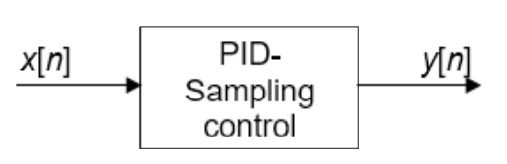
\includegraphics[width=5cm, height=2cm]{Images/image151.png}
    %\caption{}
    \label{fig:Fig 104}
    \end{figure}
    
\begin{equation}
	[y[n]=\sum _{i=1}^{M}a_{i} \cdot y[n-i] +\sum _{k=0}^{N}b_{k} \cdot x[n-k]]
\label{EQ }
\end{equation}

a common direct form (here, with input sequence \textit{x${}_{d}$}[\textit{n}] = \textit{x}[\textit{n}]) \\

The coefficients for the des PID algorithm \eqref{GrindEQ__3_5_} thus define the coefficients of an  IIR (Infinite Impulse Response) filter of 2. order

\begin{equation*}
	a_1=-1,\ a_2=0,\ b_0=k_R \cdot \left(1+\frac{T_V}{T_S}\right),\ b_1=-k_R \cdot \left(1-\frac{T_s}{T_N}+2 \frac{T_V}{T_S}\right),\ b_2=k_R \cdot \frac{T_V}{T_S}
\label{EQ }
\end{equation*}

\begin{equation*}
	y[n] = {\sum_{k=0}^{2}b_{k} \cdot x[n-k] - \sum_{i=1}^{1}a_{i} \cdot y[n-i] +} \\ = b_{0} \cdot x[n]+b_{1} \cdot x[n-1]+b_{2} \cdot x[n-2] - a_{1} \cdot y[n-1]
\label{EQ }
\end{equation*}

A digital filter on 2. order in direct form can be represented as signal flow for time discrete signals (sequences), with triangles for multiplication with coefficients, the z${}^{-1\ \ }$rectangles the delay elements for 1 sample and the circles represent additions.

	\begin{figure}[h]
    \centering
    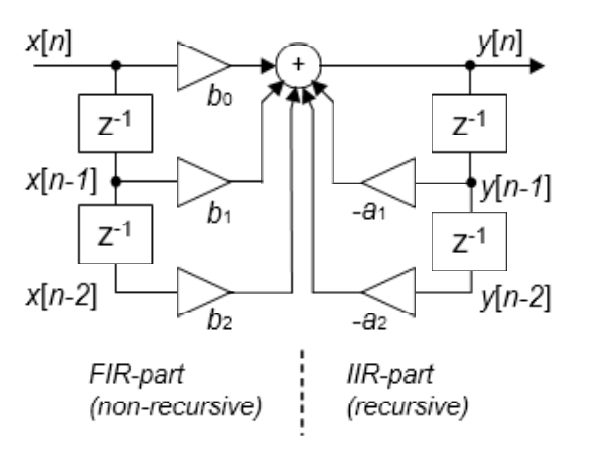
\includegraphics[width=8cm, height=4cm]{Images/image152.png}
    %\caption{}
    \label{fig:Fig 105}
    \end{figure}

The algorithm (3.8) calculates a new output value \textit{y}[\textit{n}], for each new sampling period \textit{T${}_{S}$} with a new input value \textit{x}[\textit{n}] and two previous input values \textit{x}[\textit{n}-1] and \textit{x}[\textit{n}-2] and the last output value \textit{y}[\textit{n}-1], which is stored.\\

For calculating digital filters on microcontrollers, it is generally advantageous to use optimized libraries (if available), which respect the specifics of the processor CPU. With optimizing digital filter algorithms significant reductions in execution time can be achieved ( see 3.2.1).\\

{\rot\bf PID Algorithm in C }\\

The algorithm (3.8) can be programmed in its general form in floating-point arithmetic easily with the C programming language:

\begin{itemize}
\item  \textbf{IIR2}() realizes (3.8), which is the actual digital filter, and, buffering of the 2 past output values \textit{y}[\textit{n}-1] and \textit{y}[\textit{n}-2]

\item  \textbf{store\_xd}() realizes the control difference \textit{x${}_{d}$}[\textit{n}] from the current process value \textit{x}[\textit{n}] and setpoint \textit{w}[\textit{n}]. store\_xd() also realizes the buffering of the 3 controller input values \textit{x${}_{d}$}[\textit{n}], \textit{x${}_{d}$}[\textit{n}-1], \textit{x${}_{d}$}[\textit{n}-2]

\item  \textbf{init\_pid()} calculates from a given set of controller parameters \textit{k${}_{R}$}, \textit{T${}_{N}$}, und \textit{T${}_{V}$} with the constant sampling period \textit{T${}_{S}$} a set of filter coefficients \textit{a\_}pid[] und  b\_pid[] by (3.8)
\end{itemize}

\begin{lstlisting}[style=mystyle, language=c]
// ----------------------------------------
float a_pid[3], b_pid[3], xd[3] = {0., 0., 0.}, y[3] = {0., 0., 0.}, w = 0.;
// ----------------------------------------
void init_pid(float a[], float b[], float kr, float Tn_Ts, float Tv_Ts)
{
  a[0] = a[2] = 0.0;  // Tn_Ts = Tn / Ts
  a[1] =  1.0;        // Tv_Ts = Tv / Ts
  b[0] =  kr*(1.0 + Tv_Ts);
  b[1] = -kr*(1.0 - 1.0/Tn_Ts + 2.0*Tv_Ts);
  b[2] =  kr*Tv_Ts;
}

// ----------------------------------------
void store_xd(float x0, float w)
{
  xd[2] = xd[1];    // xd*z^(-2)
  xd[1] = xd[0];    // xd*z^(-1)
  xd[0] = w-x0;   // xd*z^(0)
}

// ----------------------------------------
float IIR2(float x[],float y[],float a[],float b[])
{ // --- IIR 2nd order x[n] -> (a,b) -> y[n] 
  float sum;

  // non-recursive (FIR) section
  sum = x[0]*b[0] + x[1]*b[1] + x[2]*b[2];

  // shift output buffer values
  y[2] = y[1];  // y*z^(-2)
  y[1] = y[0];  // y*z^(-1)

  // recursive (IIR) section
  sum += y[1]*a[1] + y[2]*a[2];

  return y[0] = sum;  // y*z^(0)
}
\end{lstlisting}

It should be noted, that the use of floating-point arithmetic in microcontrollers without hardware floating-point unit usually results in large execution times, and is therefore usually avoided entirely $\rightarrow$ use \textbf{integer arithmetic} ( 3.2.1) with less powerful microcontrollers !\\

As real-time software realization, it can be favorable, to calculate the FIR and the IIR filter parts by concurrent tasks, which can then be run simultaneously on a multiprocessor hardware.\\

{\rot\bf Requirements for the Digital PID-Controller}\\

Since this controller is a digital sampling system, it must respect the requirements of the sampling theorem on the strict periodicity with \textit{T${}_{s}$} with sampling of the control variable \textit{x} and the output of the actuating variable \textit{y}. \\

For the input signal, an AD converter, either working as SAR (usually integrated on microcontrollers) or as flash type, a good strategy for getting an ADC value within the strict timing must be found (starting conversion, waiting on the result).

\begin{enumerate}

\item  Events with period \textit{T${}_{s}$} and with \textbf{minimal} deviation (\textbf{jitter}) must be produced  definition of a timer event (Ts)

\item  start of AD conversion for the \textbf{input} must occur immediately after the Ts-event,  \textbf{minimal jitter}, (limited by the specified interrupt latency).

\item  The \textbf{output} value must be DA converted (with a delay of exactly one sampling period), with minimal jitter aas with AD conversion. 

\item  It is important to ensure that the algorithm operates only with a \textbf{consistent set} of parameters and input and output buffers with consistent values. 

\item  The \textbf{controller parameters} must be \textbf{adjustable} from outside (e.g. by asynchronous bus event). The latency time allowed for a complete switch of the parameters is 100·\textit{T${}_{s}$}.It must be ensured, that any parameter change, always results with a stable digital filter. 

\item  The set value must be adjustable from outside (e.g. by asynchronous bus event). The latency time allowed here is 20·\textit{T${}_{s}$}.

\item  The real-time program shall be executable with any type of task scheduling. 
\end{enumerate}

{\rot\bf Task Definition}\\

A real-time program with 4 tasks can meet the specified requirements:

\begin{itemize}
\item  \textbf{Task T1}: a high-priority task, which controls the timing conditions for reading the input from the AD converter and writing the output to the DA converter. (wait on periodic timer event \textbf{Ev\_Ts})

\item  \textbf{Task T2}: a medium priority task, which performs the calculation of the output sample by the IIR algorithm, after a new input value is ready. Task 2 may run only when task 1 is finished $\rightarrow$ event \textbf{Ev\_12}.

\item  \textbf{Task T3}: an asynchronous low-priority task, which performs the conversion and modified PID control parameters and provides a consistent set of IIR filter coefficients $\rightarrow$ event \textbf{Ev\_par}.

\item  \textbf{Task T4}: an asynchronous low-priority task, which lets change the set value$\rightarrow$ event \textbf{Ev\_w}
\end{itemize}

{\rot\bf Critical Data}

\begin{itemize}
\item \textbf{ w (set value)}: read by T1 and can be concurrently written by T4 $\rightarrow$ Mutex \textbf{Mw}

\item \textbf{ a\_pid, b\_pid PID filter coefficients}: These are calculated and read by T2, concurrently written by T3  $\rightarrow$ Mutex \textbf{Mab}
\end{itemize}

Although the input buffer xd[], and the buffer of output values y[] is accessed by the two tasks T1 and T2, it is guaranteed by the order synchronization of T1-T2, that there will be no conflict, even without a mutex.\\

{\rot\bf  Realization of a Digital PID Control with 4 Tasks}

	\begin{figure}[h]
    \centering
    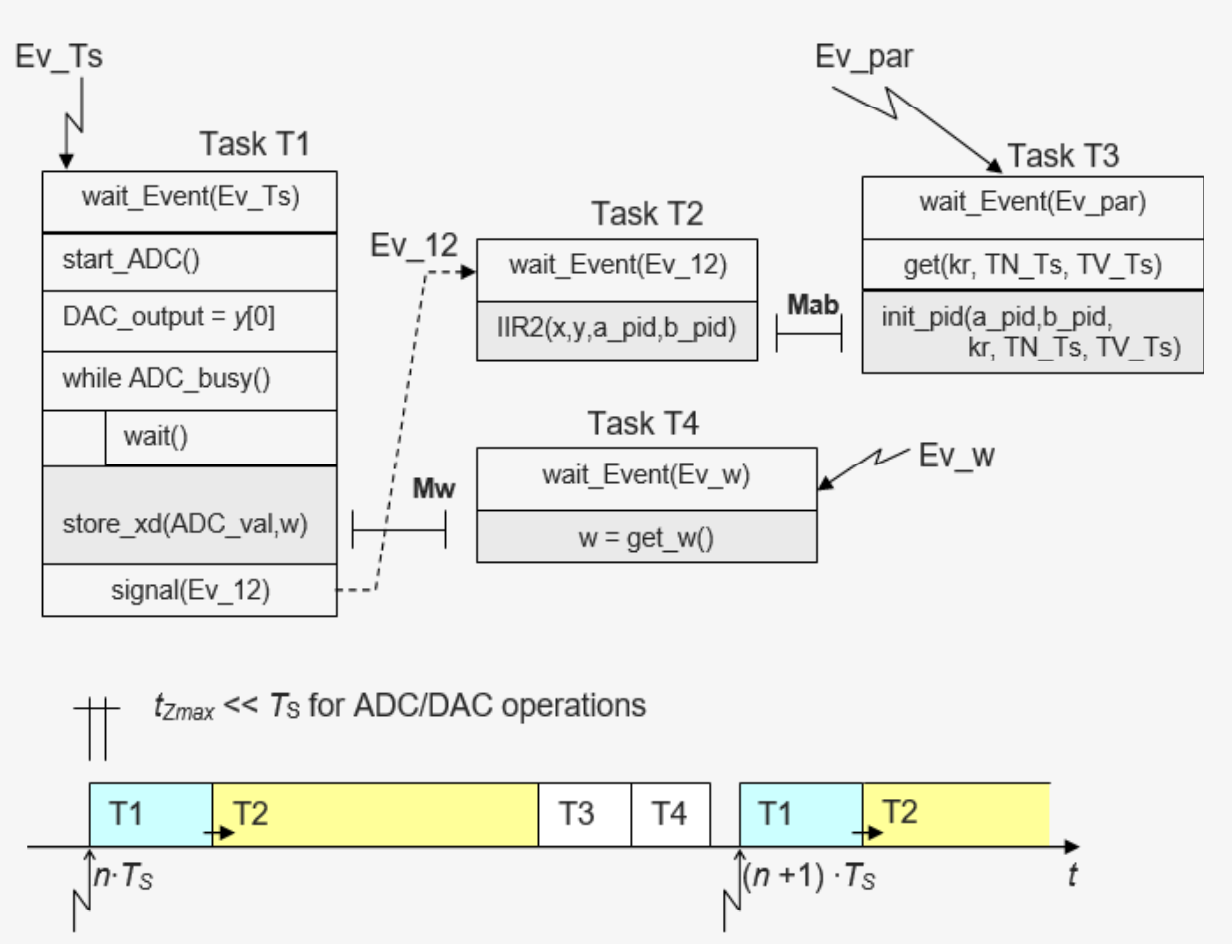
\includegraphics[width=13cm, height=7cm]{Images/image154.png}
    %\caption{}
    \label{fig:Fig 106}
    \end{figure}

This real-time program 

\begin{itemize}
\item  assures with T1: compliance with the strict time conditions for the two sampling systems ADC$\rightarrow$\textit{x}[0] and \textit{y}[0]$\rightarrow$DAC: called periodically with minimal jitter.

\item  by \textbf{Ev\_T12} is ensured, that T2 runs only when T1 is finished (cooperation sync)

\item  by Mutex \textbf{Mab is} ensured, that the PID algorithm is executed only with a consistent set of parameters.

\item  assumption is, that the utilization of task 2 was determined by measuring WCET to be \textit{H}${}_{2}$ $\mathrm{\approx}$ 50\%. If \textit{H}${}_{2\ }$is too large, optimizations are necessary (e.g. integer arithmetic) 
\end{itemize}
\newpage
\textbf{Exercise 1:} Write C Code for Realizing Task T2 under FreeRTOS.\\

- develop by re-factoring PingPong, realize Ts = 2 ms

\begin{lstlisting}[style=mystyle, language=c]
/* ----------------------------------------------------------------
   iir2.c: Module for realization of a digital filter, 2. order
   ----------------------------------------------------------------*/
// ----------------------------------------
float a_pid[3], b_pid[3], xd[3] = {0., 0., 0.}, y[3] = {0., 0., 0.}, w = 0.;
// ----------------------------------------
float IIR2(float x[],float y[],float a[],float b[])
{ // --- IIR 2nd order x[n] -> (a,b) -> y[n] 
  float sum;
  // non-recursive (FIR) section
  sum = x[0]*b[0] + x[1]*b[1] + x[2]*b[2];
  // shift output buffer values
  y[2] = y[1];  // y*z^(-2)
  y[1] = y[0];  // y*z^(-1)
  // recursive (IIR) section
  sum += y[1]*a[1] + y[2]*a[2];
  return y[0] = sum;  // y*z^(0)
}

// ----------------------------------------------------------------------------
// ----------------------------------------------------------------------------
#include "FreeRTOS.h"
xSemaphore sEv_12, siir;                   	// Semaphore sEv_12, Mutex siir
// ----------------------------------------------------------------------------
void vT2(void * pvParameters)						// re-factored vPingTask
{	
	while(1) {
		xSemaphoreTake(sEv_12,portMAX_DELAY);	// on Event Ev_12
		xSemaphoreTake(siir,portMAX_DELAY);		// acquire mutex
		IIR2(xd, y, a, b);							// Filter operation
		xSemaphoreGive(siir);						// release mutex
	}
}

// ----------------------------------------------------------------------------
void vT1(void * pvParameters)					// re-factored vPrintTask
{	
	short ADC_in;
	portTickType xLastWakeTime;
	xLastWakeTime = xTaskGetTickCount();

	while(1) {
 		vTaskDelayUntil(&xLastWakeTime, 2*configTICK_RATE_HZ/1000);  	// exact periodic Ts = 2 ms 		
		ADC_start();    				// start AD (--> SAR sample & hold) ...
		...								// busy waiting stuff here (like DAC outputs)
		while(ADC_busy());			// wait for ADC (some microseconds) ...
		ADC_in = ADC_get(); 			// store ADC result				
		update_x_buffer(ADC_in);	// update the filter input buffer xd[]
		xSemaphoreGive(sEv_12);  	// sync to task T2
	}	
}
\end{lstlisting}
\newpage

\textbf{Exercise 2: }PI controller (for ATmega microcontrollers)

\begin{enumerate}
\item Design a real-time program for a PI controller with the non-preemptive binary fixed time-slice method (FTS) for the following parameters \\ execution times: \textit{T}${}_{e1}$ = 50 $\mu$s, \textit{T}${}_{e2}$ = 300 $\mu$s, \textit{T}${}_{e3}$ = 100 $\mu$s, \textit{T}${}_{e4}$ = 50 $\mu$s.\\ - T3 und T4 shall be able to process asynchronous events about 20 times per sec.\\- the initial control parameters: \textit{k${}_{R}$} = 5, \textit{T${}_{N}$} = 20 ms.
\item Determine a new Schedule for the case where due to halving of the clock frequency of the micro-controller, each task has approximately twice the execution time of (1).
\end{enumerate}

\textbf{Solution:}

\begin{enumerate}
\item \textit{H}${}_{1}$ = 5 \%, \textit{H}${}_{2}$ = 30 \%, \textit{H}${}_{3}$ = 0.1/20 = 0.5 \%, \textit{H}${}_{4}$ = 0.05/20 = 0.25 \%  \textit{H} = 30.75 \%\\

with 3 tasks, non-preemptive binary time-slice scheduler with \textit{T${}_{TS}$} $\mathrm{\ge}$ max(\textit{T${}_{ei}$}), \\
$\rightarrow$ periodic timer events with basic time-slice\textit{ T${}_{TS}$} = 0.5 ms, so execution times of each of the 4 tasks are below the maximum possible execution time of the basic time-slice.\\
 
 	\begin{figure}[h]
    \centering
    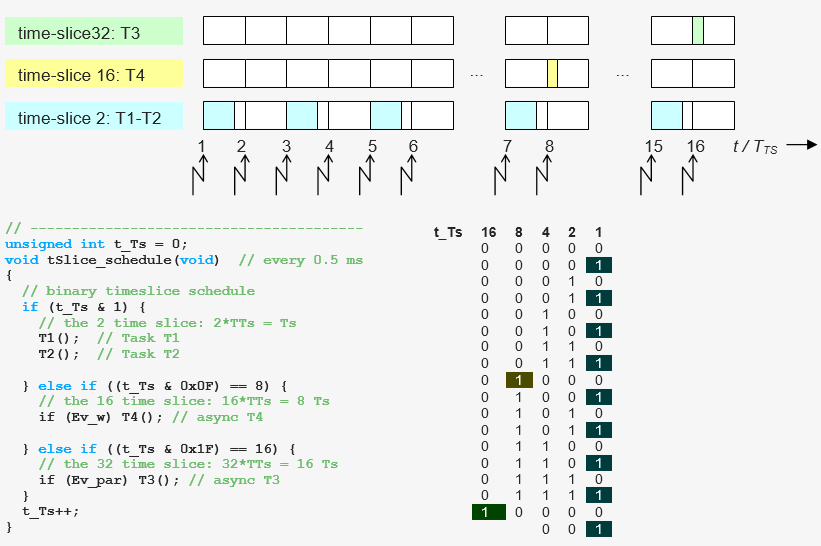
\includegraphics[width=14cm, height=9cm]{Images/image156.png}
    %\caption{}
    \label{fig:Fig 107}
    \end{figure}
    
\begin{itemize}
\item T1 and T2 run successively (no sync needed) in the time-slice called every 2 times
\item T4 runs every 8 ms (= time-slice 16)
\item T3 runs every 16 ms (= time-slice 32), all synchronous to the periodic timer events
\item the execution times of all 4 tasks are well below the maximum time $T_{TS}$ = 0.5 ms.
\end{itemize}

\item  Doubled execution time (e.g. due to reduction of the CPU clock frequency)\\  \textit{T}${}_{e1}$ = 100 $\mu$s, \textit{T}${}_{e2}$ = 600 $\mu$s, \textit{T}${}_{e3}$ = 200 $\mu$s und \textit{T}${}_{e4}$ = 100 $\mu$s\textit{ }\\

\textit{ H}${}_{1}$ = 10 \%, \textit{H}${}_{2}$ = 60 \%, \textit{H}${}_{3}$ = 0.2/20 = 1 \%, \textit{H}${}_{4}$ = 0.1/20 = 0.5 \%  \textit{H} = 71.5 \%\\

Solution:\\
with 3 tasks, non-preemptive binary time-slice scheduler with \textit{T${}_{TS}$} $\mathrm{\ge}$ max(\textit{T${}_{ei}$}), \\

$\rightarrow$ periodic timer events with basic time-slice \textit{T${}_{TS}$} = 1.0 ms, so execution times of each of the 4 tasks are below the maximum possible execution time of the basic time-slice.

	\begin{figure}[h]
    \centering
    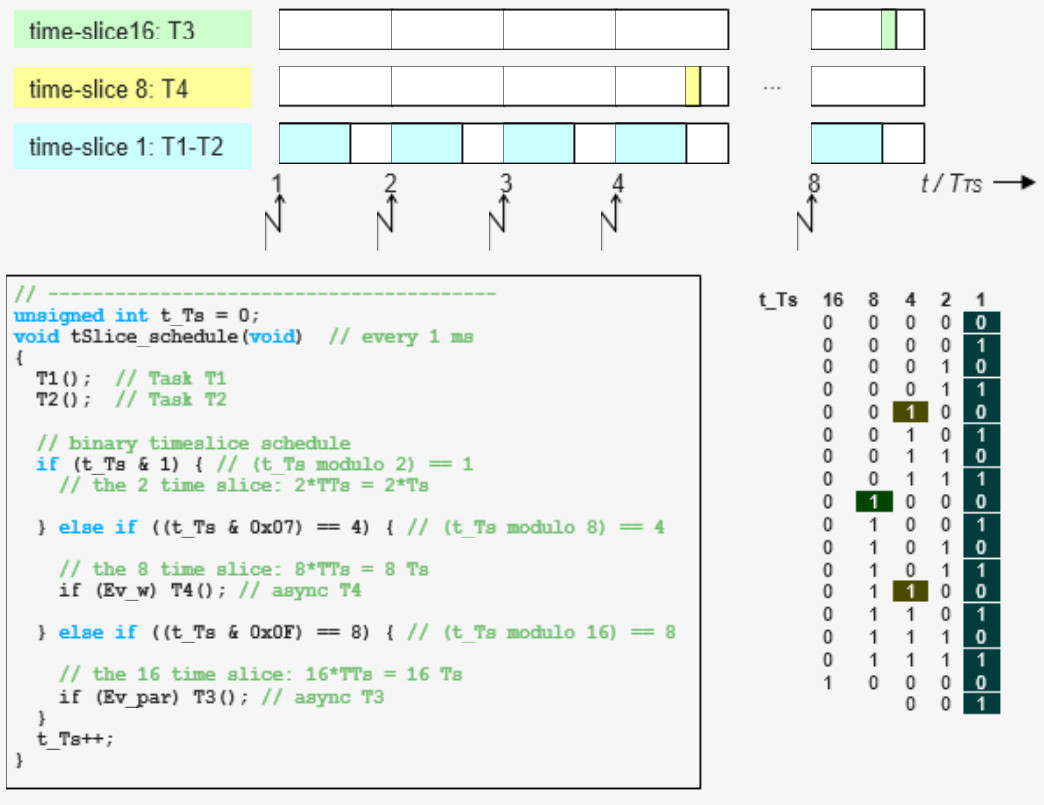
\includegraphics[width=14cm, height=9cm]{Images/image157.png}
    %\caption{}
    \label{fig:Fig 108}
    \end{figure}
   
\begin{itemize}
\item T4 runs every 8 ms (time-slice 8)
\item T3 runs every 16 ms (time-slice 16), both asynchronous to the periodic timer events  (after T1-T2) !
\item The maximum execution time is within time-slice 8: $T_{e1}$ + $T_{e2}$ + $T_{e3}$ = 900 $\mu$s.
\end{itemize}
\end{enumerate} 
\newpage 

\section{Finite State Machines (FSM)}

In most embedded applications finite state machines are used to interface with non-synchronous, periodic devices, such as switches, slow actuators, indication lamps, networks {\dots} \\

Traditional event-based programming is used with modern GUI based standard OS, Windows, Linux, .. with both desktop and portable applications handling keyboard mouse, touchpanels, {\dots} as inputs as well as with networks.$\rightarrow$  https://en.wikipedia.org/wiki/Automata-based\_programming\\

	\begin{figure}[h]
    \centering
    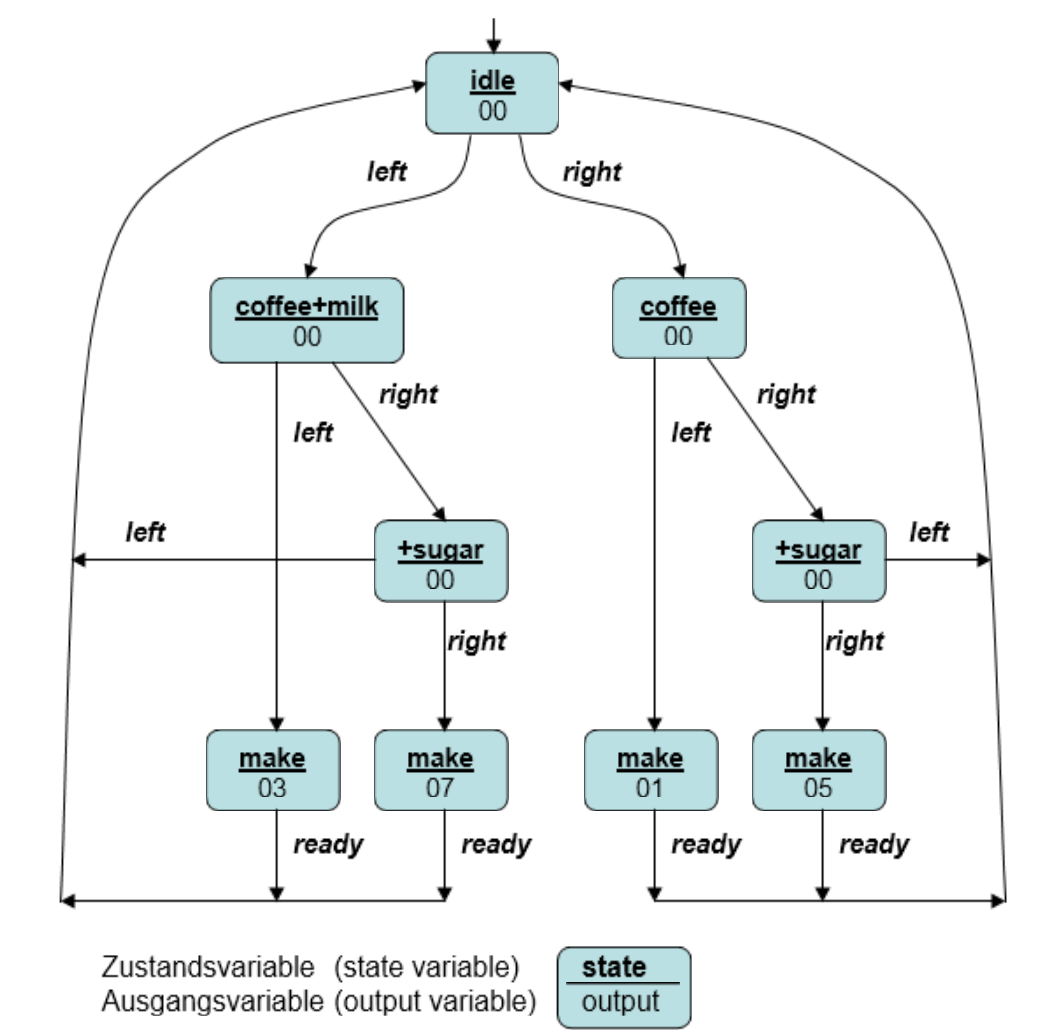
\includegraphics[width=14cm, height=12cm]{Images/image158.png}
    \caption{Finite State Machines (FSM)}
    \label{fig:Fig 109}
    \end{figure}                   

Moore Finite State Machine: Each state has assigned exactly one output. \\
\newpage
\textbf{Coffee Automat: State Transient Table}

	\begin{figure}[h]
    \centering
    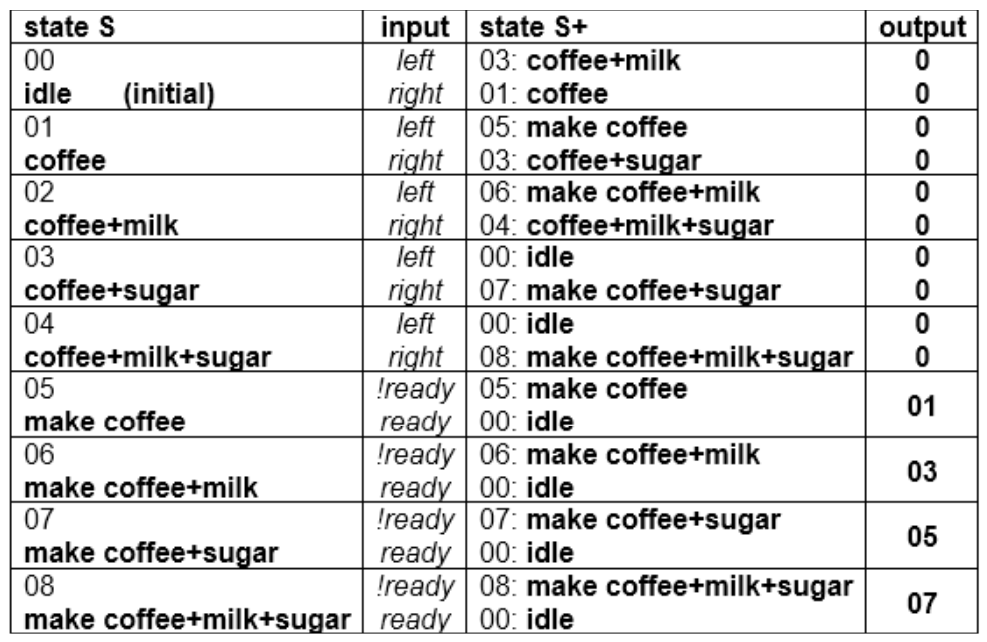
\includegraphics[width=12cm, height=8cm]{Images/image186.png}
    %\caption{Finite State Machines (FSM)}
    \label{fig:Fig 110}
    \end{figure} 
     
\textbf{Coffee Automat: Implementation in C	 ($\rightarrow$ ProgC\ \ FSM\_CoffeeAutomat)}\\

\begin{lstlisting}[style=mystyle, language=c]
// ----------------------------------------------------------------------------
// the FSM states for the Coffee Automata
// ----------------------------------------------------------------------------
enum {	FSM_STATE_IDLE, 	
			FSM_STATE_COFFEE, 						FSM_STATE_COFFEE_MILK, 
			FSM_STATE_COFFEE_SUGAR, 			FSM_STATE_COFFEE_MILK_SUGAR, 
			FSM_STATE_MAKE_COFFEE, 				FSM_STATE_MAKE_COFFEE_MILK, 
			FSM_STATE_MAKE_COFFEE_SUGAR, 	FSM_STATE_MAKE_COFFEE_MILK_SUGAR, 
};
// ----------------------------------------------------------------------------
int fsm_state = FSM_STATE_IDLE;
// ----------------------------------------------------------------------------

// ----------------------------------------------------------------------------
// the FSM outputs, one for each state, (Moore Automata model)
// ----------------------------------------------------------------------------
const int fsm_output[NUM_FSM_STATES] = { 	// output is fsm_output[fsm_state]
		0,												// bit0: add coffee
		0,	0,											// bit1: add milk
		0,	0,											// bit2: add sugar
		1,	3,
		5,	7
 };

// ----------------------------------------------------------------------------
// the FSM inputs
// ----------------------------------------------------------------------------
enum {	FSM_INP_NONE=0, FSM_INP_LEFT, FSM_INP_RIGHT, FSM_INP_READY 
// ----------------------------------------------------------------------------
int fsm_tic(int fsm_inp) 		// called periodically, e.g. each 50 ms
{
	// ------------------------------------------------------------
	// the FSM transients, realizing the state transient table
	// ------------------------------------------------------------
	switch (fsm_state) {
	case FSM_STATE_IDLE:
		if (fsm_inp == FSM_INP_LEFT) fsm_state = FSM_STATE_COFFEE;
		if (fsm_inp == FSM_INP_RIGHT) fsm_state = FSM_STATE_COFFEE_MILK;
		break;
		
	case FSM_STATE_COFFEE:
		if (fsm_inp == FSM_INP_LEFT) fsm_state = FSM_STATE_MAKE_COFFEE;
		if (fsm_inp == FSM_INP_RIGHT) fsm_state = FSM_STATE_COFFEE_SUGAR;
		break;

	case FSM_STATE_COFFEE_MILK:
		if (fsm_inp == FSM_INP_LEFT) fsm_state = FSM_STATE_MAKE_COFFEE_MILK;
		if (fsm_inp == FSM_INP_RIGHT) fsm_state = FSM_STATE_COFFEE_MILK_SUGAR;
		break;

	case FSM_STATE_COFFEE_SUGAR:
		if (fsm_inp == FSM_INP_LEFT) fsm_state = FSM_STATE_IDLE;
		if (fsm_inp == FSM_INP_RIGHT) fsm_state = FSM_STATE_MAKE_COFFEE_SUGAR;
		break;

	case FSM_STATE_COFFEE_MILK_SUGAR:
		if (fsm_inp == FSM_INP_LEFT) fsm_state = FSM_STATE_IDLE;
		if (fsm_inp == FSM_INP_RIGHT) fsm_state = FSM_STATE_MAKE_COFFEE_MILK_SUGAR;
		break;

	case FSM_STATE_MAKE_COFFEE:
	case FSM_STATE_MAKE_COFFEE_MILK:
	case FSM_STATE_MAKE_COFFEE_SUGAR:
	case FSM_STATE_MAKE_COFFEE_MILK_SUGAR:
		if (fsm_inp == FSM_INP_READY) fsm_state = FSM_STATE_IDLE;
		break;

	default:
		;		// no state change
	}
	OUTPUT(fsm_output[fsm_state]);		// Moore FSM: one output per state
	return 
\end{lstlisting}

The above implementation in C is optimized for readability rather than for minimum runtime or memory ressources. However, the above code uses very little memory space and is running quite fast.

\begin{tcolorbox}[colback=blue!5!white,colframe=blue!75!black]
Recipe for Realizing an FSM in C  (Moore FSM)
\begin{itemize}
\item Analyze the problem before coding, plot a state diagram, define the states
\item Use enums to encode states in a well readable form
\end{itemize}
\end{tcolorbox}

\begin{itemize}
\item Define outputs as enums with suitable encoding, e.g. as bit-fields
\item Define input conditions causing the state transitions as enums as well
\item Realize a periodicaly called fsm\_tic function, realize transients and outputs
\end{itemize}

\textbf{Exercise:} Develop a Traffic-Light including yellow phases from section 1.2 as a Moore-FSM as the above Coffee Automat with C-Code. The yellow phases shall last 2 s, the main green/red phases shall be 8 s each. Assume the fsm\_tic() is called with 1 s periodic time. Plot a State Diagram and the state transient table.

	\begin{figure}[h]
    \centering
    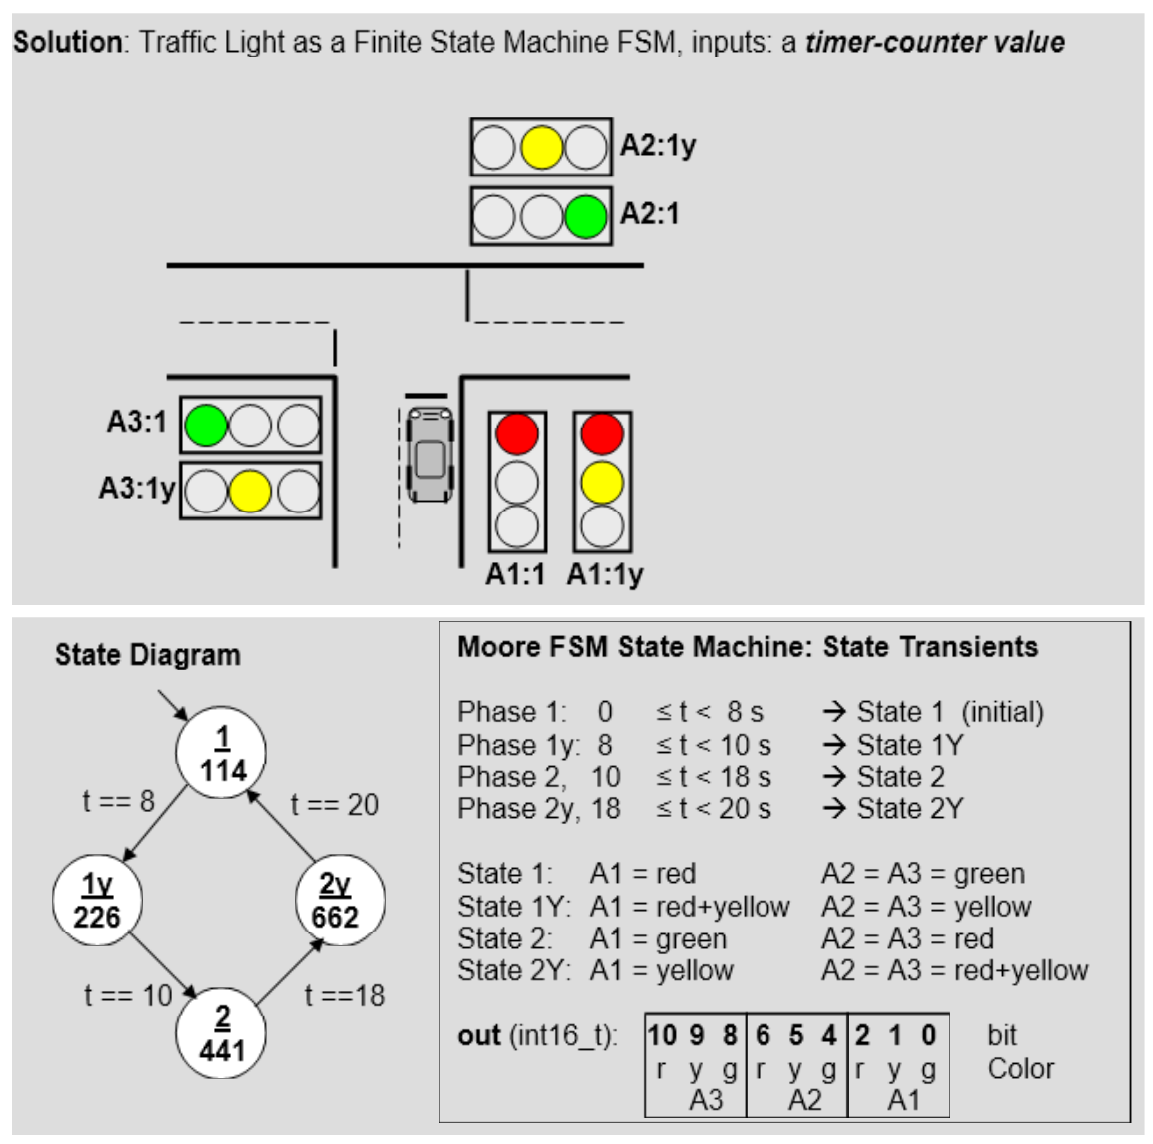
\includegraphics[width=15cm, height=12.5cm]{Images/image159.png}
    %\caption{}
    \label{fig:Fig 111}
    \end{figure}

{\rot\bf C-Code	($\rightarrow$ ProgC \ FSM\_TrafficLight)}\\

\begin{lstlisting}[style=mystyle, language=c]
// ----------------------------------------------------------------------------
// the FSM states, here for the TrafficLight
// ----------------------------------------------------------------------------
enum fsm_state_e {
		FSM_STATE_1=0, 						FSM_STATE_1Y,
		FSM_STATE_2, 						FSM_STATE_2Y,
		NUM_FSM_STATES
};

// ----------------------------------------------------------------------------
// the FSM state
// ----------------------------------------------------------------------------
int fsm_state = FSM_STATE_1;	// initial state
int fsm_count = 0;					// the FSM counter

// ----------------------------------------------------------------------------
// the FSM outputs, bit assignments, one for each state (Moore)
// ----------------------------------------------------------------------------
enum fsm_out_e {	FSM_OUT_A1_G=1, 	FSM_OUT_A1_Y=2, 	FSM_OUT_A1_R=4,
							FSM_OUT_A2_G=0x10, 	FSM_OUT_A2_Y=0x20, 	FSM_OUT_A2_R=0x40,
							FSM_OUT_A3_G=0x100, FSM_OUT_A3_Y=0x200, FSM_OUT_A3_R=0x400,
							NUM_FSM_OUTPUTS };

const int fsm_output[NUM_FSM_STATES] = {				// output is fsm_output[fsm_state]
		FSM_OUT_A1_R|FSM_OUT_A2_G|FSM_OUT_A3_G,		// output with FSM_STATE_1
		FSM_OUT_A1_R|FSM_OUT_A1_Y|FSM_OUT_A2_Y|FSM_OUT_A3_Y,	// output with FSM_STATE_1Y
		FSM_OUT_A1_G|FSM_OUT_A2_R|FSM_OUT_A3_R,		// output with FSM_STATE_2
		FSM_OUT_A2_Y|FSM_OUT_A2_R|FSM_OUT_A3_R
					|FSM_OUT_A2_Y|FSM_OUT_A3_Y				// output with FSM_STATE_2Y
};

// ----------------------------------------------------------------------------
#define T_RED_GREEN	8	// Time for Red/Green phases in Ts
#define T_YELLOW	2		// Time for Yellow    phases in Ts
// ----------------------------------------------------------------------------
int fsm_tic()
{
	// ------------------------------------------------------------
	// the FSM 
	// ------------------------------------------------------------
	if (fsm_count < T_RED_GREEN)
		fsm_state = FSM_STATE_1;
	else if (fsm_count < (T_RED_GREEN + T_YELLOW))
		fsm_state = FSM_STATE_1Y;
	else if (fsm_count < (2*T_RED_GREEN + T_YELLOW))
		fsm_state = FSM_STATE_2;
	else if (fsm_count < (2*T_RED_GREEN + 2*T_YELLOW))
		fsm_state = FSM_STATE_2Y;
	else {
		fsm_state = FSM_STATE_1;
		fsm_count = 0;	// modulo cycle time
	}
	// ------------------------------------------------------------
	fsm_out();					// Moore FSM: one output per state
	// ------------------------------------------------------------
	fsm_count ++;
	return fsm_state;
}

// ----------------------------------------------------------------------------
int main()
{
	int ch;
	gotoXY(0,0);
  		printf("Traffic light, Ctrl-Break: exit");
    	do {	// basic terminal loop
        ch = 0;
        if ( kbhit() ) {
            ch = getch();
        }
			fsm_tic();			// fsm tick
        Sleep(1000);		// Ts = 1000 ms

    } while ( ch != 127);	// until user hits ctrl-backspace.
	return 

\end{lstlisting}


